\documentclass[11pt]{article}
\usepackage{amsmath, amssymb, amsfonts,  graphicx, enumerate, float, wrapfig, hyperref}
\usepackage[margin=0.5in]{geometry}
\graphicspath{{./}}
\newcommand*{\vs}{\vspace{1cm}}
\newcommand*{\next}{\noindent}
\newcommand*{\set}{\setcounter{equation}{0}}

\begin{document}

\title{3.9 Differentials}
\author{Juan J. Moreno Santos}
\date{November 2023}

\maketitle
\section{Find the equation of the tangent line $T$ to the graph of $f$ at the given point. Use this linear approximation to complete the table.}
2.\begin{align}
    f(x)&=\frac{6}{x^2},\,\,\left(2,\,\,\frac{3}{2}\right)\\
    f(x)&=6x^{-2}\\
    f'(x)&=-12x^-3=\frac{-12}{x^3}\\
\end{align}
Find the tangent line:
\begin{align}
    y-\frac{3}{2}&=\frac{-12}{8}(x-2)\\
    &=\frac{-3}{2}(x-2)\\
    y&=-\frac{3}{2}x+\frac{9}{2}
\end{align}

\begin{flushleft}
    \begin{table}[h]
        \begin{tabular}{|l|l|l|l|l|l|}
        \hline
            x & 1.9 & 1.99 & 2 & 2.01 & 2.1\\\hline
            $f(x)=\frac{6}{x^2}$ & 1.6620 & 1.5151 & 1.5 & 1.4851 & 1.3605\\\hline
            $T(x)=-\frac{3}{2}x+\frac{9}{2}$ & 1.65 & 1.515 & 1.5 & 1.485 & 1.35\\
        \hline
        \end{tabular}
    \end{table}
\end{flushleft}

\vs\next
6.\begin{align}
    \set
f(x)&=\csc x,\,\,(2,\csc 2)\\
f'(x)&=-\csc x\cot x\\
\end{align}
Find the tangent line:
\begin{align}
y-f(2)&=f'(2)(x-2)\\
y-\csc 2&=(-\csc 2\cot 2)(x-2)\\
y&=(-\csc 2\cot 2)(x-2)+\csc 2
\end{align}

\begin{flushleft}
    \begin{table}[h]
        \begin{tabular}{|l|l|l|l|l|l|}
        \hline
            x & 1.9 & 1.99 & 2 & 2.01 & 2.1\\\hline
            $f(x)=\csc x$ & 1.0567 & 1.0948 & 1.0998 & 1.1049 & 1.158\\\hline
            $T(x)=(-\csc 2\cot 2)(x-2)+\csc 2$ & 1.0494 & 1.0947 & 1.0998 & 1.1048 & 1.1501\\
        \hline
        \end{tabular}
    \end{table}
\end{flushleft}

\section{Use the information to evaluate and compare $\Delta y$ and $dy$.}
8.\begin{align}
    \set
    y&=1-2x^2,\,\, x=0,\,\, \Delta x=dx=-0.1\\
    y'&=-4x\\
    \Delta y&=f(x+\Delta x)-f(x)\\
    &=f(-0.1)-f(0)\\
    &=(1-2(-0.01)^2)-(1-2(0)^2)\\
    &=-0.02\\
    dy&=f'(x)dx\\
    &=f'(0)(-.01)\\
    &=(0)(-0.1)\\
    &=0
\end{align}

\next
10.\begin{align}
    \set
    y&=2-x^4,\,\, x=2,\,\, \Delta x=dx=0.01\\
    f'(x)&=-4x^3\\
    \Delta y&=f(2.01)-f(2)\\
    &\approx -14.3224-(-14)=-0.3224\\
    dy&=(-4x^3)dx\\
    &=-4(2)^3(0.01)\\
    &=-0.32
\end{align}

\section{Find the differential $dy$ of the given function.}
14.\begin{align}
    \set
    y&=\sqrt[]{9-x^2}\\
    dy&=\frac{1}{2}(9-x^2)^{-1/2}dx\\
    &=\frac{-x}{\sqrt[]{9-x^2}}dx
\end{align}

\next
18\begin{align}
    \set
    y&=x\cos x\\
    dy&=(-x\sin x+\cos x)dx
\end{align}

\section{Use differentials and the graph of $f$ to approximate (a)$f(1.9)$ and (b)$f(2.04)$.}
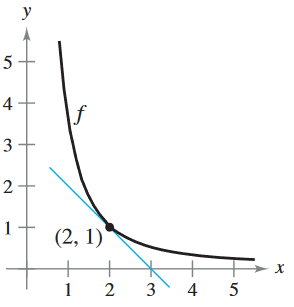
\includegraphics{22.png}\\
22.\begin{enumerate}[(a)]
    \item
        \begin{align}
        \set
        f(1.9)&=f(2.-0.1)\\
        &\approx f(2)+f'(2)(0.04)\\
        &\approx 1+(-1)(-0.1)\\
        &=1.1            
        \end{align}
    \item
        \begin{align}
        f(2.04)&=f(2+0.04)\\
        &\approx f(2)+f'(2)(0.04)\\
        &\approx 1+(-1)(0.04)\\
        &=0.96
        \end{align}
\end{enumerate}

\section{Use the differentials and the graph of $g'$ to approximate (a)$g(2.93)$ and (b)$g(3.1)$ given that $g(3)=8$.}
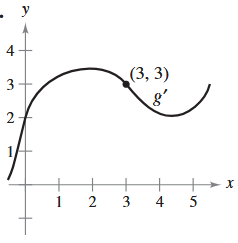
\includegraphics{26.png}\\
26.\begin{enumerate}[(a)]
    \item
        \begin{align}
        \set
        g(2.93)&=g(3-0.07)\\
        &\approx g(3)+g'(3)(-0.07)\\
        &\approx 8+(3)(-0.07)\\
        &=7.79
        \end{align}
    \item 
        \begin{align}
        \set
        g(3.1)&=g(3+0.1)\\
        &\approx g(3)+g'(3)(0.1)\\
        &\approx 8+(3)(0.1)\\
        &=8.3
        \end{align}
\end{enumerate}

\section{Area}
28. The measurements of the base and altitude of a triangle are found to be 36 and 50 centimeters, respectively. The possible error in each measurement is 0.25 centimeter. Use differentials to approximate the possible propagated error in computing the area of the triangle.
\begin{align}
    \set
    A&=\frac{1}{2}bh,\,\, b=36,\,\, h=50\\
    db&=dh=\pm 0.25\\
    dA&=\frac{1}{2}bdh+\frac{1}{2}hdb\\
    \Delta A&\approx dA=\frac{1}{2}(36)(\pm 0.25)+\frac{1}{2}(50)(\pm 0.25)\\
    &=\pm 10.75\text{cm}^2
\end{align}

\section{Circumference}
32. The measurement of the circumference of a circle is found to be 64 centimeters, with a possible error of 0.9 centimeter.
\begin{enumerate}[(a)]
    \item Approximate the percent error in computing the area of the circle.
        \begin{align}
            \set
            C&=64\text{cm}\\
            \Delta C&=dC=\pm 0.9cm\\
            C&=2\pi r\Rightarrow r=\frac{C}{2\pi}\\
            A&=\pi r^2=\pi\left(\frac{C}{2\pi}\right)^2=\frac{1}{4\pi}C^2\\
            \frac{dA}{A}&=\frac{\frac{28.8}{\pi}}{\left(\frac{1}{4\pi}\right)(64)^2}\approx 0.028125=2.8\%\\
        \end{align}
    \item Estimate the maximum allowable percent error in measuring the circumference if the error in computing the area cannot exceed 3\%.
        \begin{align}
            \set
            \frac{dA}{A}&=\frac{\left(\frac{1}{2\pi}\right)CdC}{\left(\frac{1}{4\pi}\right)C^2}=\frac{2dC}{C}\leq 0.03\\
            \frac{dC}{C}&\leq\frac{0.03}{2}=0.015=1.5\%
        \end{align}
\end{enumerate}

\section{The thickness of each shell is 0.2 centimeter. Use differentials to approximate the volume of each shell.}
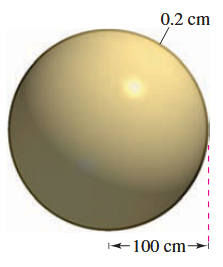
\includegraphics{36.png}
36.\begin{align}
    \set
    V&=\frac{4}{3}\pi r^3,\,\, r=100\text{cm},\,\, dr=0.2\text{cm}\\
    \Delta V&\approx dV=4\pi r^2dr=4\pi(100)^2(0.2)=8000\pi\text{cm}^3
\end{align}

\section{Surveying}
42. A surveyor standing 50 feet from a base of a large tree measures the angle of elevaton to the top of the tree as 71.5$^{\circ}$. How accurately must the angle be measured if the percent error in estimating the height of the tree is to be less than 6\%?
\begin{align}
    \set
    h&=50\tan\theta\\
    \theta&=71.5^{\circ}=1.2479\,\,\text{radians}\\
    dh&=50\sec^2\theta\cdot d\theta\\
    \left|\frac{dh}{h}\right|&=\left|\frac{50\sec^2(1.2479)}{50\tan(1.24279)}d\theta\right|\leq 0.06\\
    |d\theta|&\leq 0.018
\end{align}

\section{Use differentials to approximate the value of the expression. Compare your answer with that of a calculator.}
44.\[\sqrt[3]{26}\]
\begin{align}
    \set
    f(x)&=\sqrt[3]{x},\,\, x=27,\,\, dx=-1\\
    f(x+\Delta x)&\approx f(x)+f'(x)dx=\sqrt[3]{x}+\frac{2}{3\sqrt[3]{x^2}}dx\\
    \sqrt[3]{27}+\frac{1}{3\sqrt[3]{27^2}}(-1)&=3-\frac{1}{27}\approx \sqrt[3]{26}\approx 2.96
\end{align}
With a calculator, $\sqrt[3]{26}\approx 2.9625$.

\section{Verify the tangent line approximation of the funciton at the given point. Then use a graphing utility to graph the function and its approximation in the same viewing window.}
48.\begin{align}
   \set
   f(x)&=\tan x\\
   f'(x)&=\sec^2x\\
   f(0)&=0\\
   f'(0)&=1 
\end{align}
Tangent line at the origin:
\begin{align}
    y-0&=(x-0)\\
    y&=x
\end{align}

\section{Capstone}
52. Would you use $y=x$ to approximate $f(x)=\sin x$ near $x=0$? Why or why not?\\
\indent Yes because this is the same approximation of the function's tangent line at this point as well.

\section{Determine whether the statement is true or false. If it is false, explain why or give an example that shows it is false.}
53. If $y=x+c$, then $dy=dx$.\\
\indent True.

\vs\next
54. If $y=ax+b$, then $\frac{\Delta y}{\Delta x}$=$\frac{dy}{dx}$.\\
\indent True.

\vs\next
55. If $y$ is differentiable, then $\lim_{\Delta x\to 0}(\Delta y-dy)=0$.\\
\indent True.

\vs\next
56. If $y=f(x)$, $f$ is increasing and differentiable, and $\Delta x>0$, then $\Delta y\geq dy$.\\
\indent False. If $f(x)=\sqrt[]{x}$, $dx=3$, and $x=1$, then:
\[\Delta y=f(x+\Delta x)-f(x)=f(4)-f(1)=1\] \indent and \[dy=f'(x)dx=\frac{1}{2\sqrt[]{1}}(3)=\frac{3}{2}\]
\indent Therefore, in this particular example, $dy>\Delta y$.



























































\end{document}